%==============================================================================
% Sjabloon poster bachproef
%==============================================================================
% Gebaseerd op document class `a0poster' door Gerlinde Kettl en Matthias Weiser
% Aangepast voor gebruik aan HOGENT door Jens Buysse en Bert Van Vreckem

\documentclass[a0,portrait]{hogent-poster}

% Info over de opleiding
\course{Bachelorproef}
\studyprogramme{toegepaste informatica}
\academicyear{\advance\year by -1 \the\year-\advance\year by 1 \the\year}
\institution{Hogeschool Gent, Valentin Vaerwyckweg 1, 9000 Gent}

% Info over de bachelorproef
\title{Automatische detectie van (historische) open/gesloten status van POI’s met AI}
\author{Maxim Van Der Schueren}
\email{maxim.vanderschueren@student.hogent.be}
\supervisor{Dhr. Tom Antjon}
\cosupervisor{Dhr. Bavo Deprez (Accurat)}

% Indien ingevuld, wordt deze informatie toegevoegd aan het einde van de
% abstract. Zet in commentaar als je dit niet wilt.
\specialisation{AI \& Data Engineering}
\keywords{Point of Interest, statusdetectie, machine learning, GeoAI, POI-levenscyclus, mobiliteitsdata}
\projectrepo{https://github.com/MaximVDS/BP_Maxim_Van_Der_Schueren_2526}

\begin{document}

\maketitle
\begin{abstract}
POI-databanken vormen de basis van locatiegebaseerde analyses zoals marktstudies en concurrentie-inzicht. Een veelvoorkomend probleem is dat de operationele status van POI's in databanken vaak verouderd of onvolledig is, wat leidt tot foutieve beslissingen en de betrouwbaarheid van locatiegebaseerde toepassingen ondermijnt. De centrale onderzoeksvraag luidt: \textit{``Hoe kan artificiële intelligentie worden ingezet om automatisch de (historische) open of gesloten status van Points of Interest te detecteren, en hoe kan deze aanpak zorgen voor actuelere data in locatiegebaseerde toepassingen?''}. Om dit te onderzoeken werd een proof of concept ontwikkeld op basis van de interne POI-databank van Accurat BV voor België, Nederland, Luxemburg en Frankrijk, waarbij drie machine learning modellen werden getraind en vergeleken: Logistische Regressie, Random Forest en XGBoost. Het Random Forest model presteerde het beste met een accuracy van 76\% en een F1-score van 0.82 op een testset van 228.179 records. Dit toont aan dat automatische statusdetectie technisch haalbaar is op basis van intern beschikbare data, zonder dat dure externe databronnen vereist zijn.
\end{abstract}

\begin{multicols}{2} % This is how many columns your poster will be broken into, a portrait poster is generally split into 2 columns

\section{Introductie}

POI-databanken vormen de basis van locatiegebaseerde toepassingen zoals navigatiesoftware, marktanalyses en logistieke planning. In de praktijk is de operationele status van vestigingen er systematisch verouderd: winkels openen of sluiten zonder onmiddellijke registratie. Huidige controlemethoden zijn grotendeels handmatig, wat resulteert in een aanzienlijke vertraging tussen de daadwerkelijke status van een POI en de databank.

De centrale onderzoeksvraag van die onderzoek is: \textit{``Hoe kan artificiële intelligentie worden ingezet om automatisch de (historische) open of gesloten status van Points of Interest te detecteren, en hoe kan deze aanpak zorgen voor actuelere data in locatiegebaseerde toepassingen?''}

Het onderzoek focust zich op supermarkten als POI type, omwille van hun relevantie, hun duidelijk statusgedrag (open of gesloten) en de beschikbaarheid van voldoende publieke data.

\textbf{Deelvragen probleemdomein:}
\begin{itemize}
    \item Welke gegevensbronnen kunnen worden gebruikt voor het automatisch bepalen of een POI (historisch) open of gesloten is?
    \item Wat zijn de uitdagingen bij het implementeren van AI voor POI statusdetectie?
\end{itemize}

\textbf{Deelvragen oplossingsdomein:}
\begin{itemize}
    \item Welke AI- en machine learning technieken zijn geschikt voor de detectie van historische POI openingen en sluitingen, en wat zijn de voor- en nadelen?
    \item Hoe kan de betrouwbaarheid van automatisch gedetecteerde wijzigingen in de bedrijfstoestand van POI's worden gevalideerd?
\end{itemize}

\section{Methodologie}

Het onderzoek werd uitgewerkt in zes opeenvolgende fasen, weergegeven in figuur~\ref{fig:gantt}. De dataset werd ter beschikking gesteld door Accurat BV en bevat 1.337.279 POI-records voor België, Nederland, Luxemburg en Frankrijk. Na filtering bleven 1.140.895 bruikbare records over, met een klassebalans van 53,9\% open en 46,1\% gesloten. De dataset werd opgedeeld in een trainingsset (80\%) en testset (20\%) via een gelaagde splitsing. Drie supervised classificatiemodellen werden getraind en vergeleken — Logistische Regressie, Random Forest en XGBoost — en geëvalueerd op accuracy, precision, recall, F1-score en ROC-AUC.

\begin{center}
    \captionsetup{type=figure}
    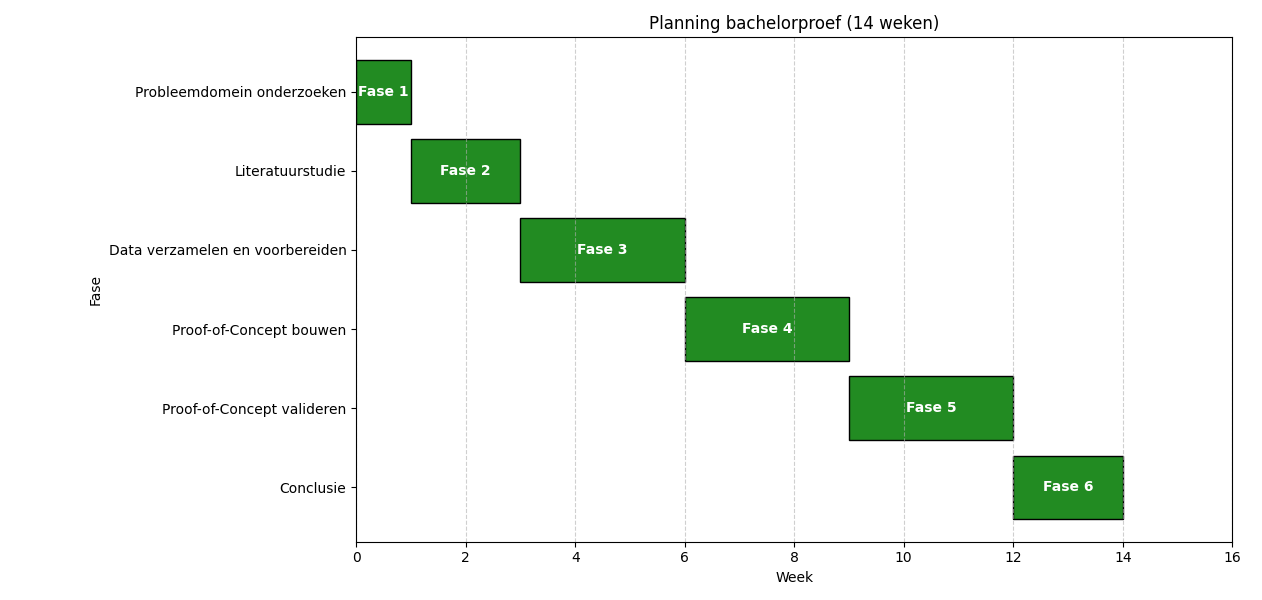
\includegraphics[width=1.0\linewidth]{./Gantt_grafiek.png}
    \captionof{figure}{Overzicht van de zes onderzoeksfasen.}
    \label{fig:gantt}
\end{center} 

\section{Uitbreiding: mobiliteitsdata}
Dynamische mobiliteitspatronen vormen volgens de literatuur een sterk aanvullend signaal voor statusdetectie. Omdat echte GPS-data echter niet beschikbaar was binnen de scope van dit onderzoek, werd een uitbreidingsexperiment opgezet. Mobiliteitsdata werd per POI gesimuleerd over 26 weken op basis van de POI-levenscyclus: een stabiele fase met realistisch weekpatroon (piek vrijdag--zaterdag), een decay-fase met lineair dalend bezoekersaantal over tien weken voor de sluiting, en een gesloten fase met nagenoeg nul bezoekers. Op POI-niveau werden drie features geaggregeerd: \texttt{gem\_bezoekers}, \texttt{std\_bezoekers} en \texttt{max\_bezoekers}.

\section{Resultaten}

\begin{center}
    \captionsetup{type=table}
    \begin{tabular}{lccccc}
        \toprule
        \textbf{Model} & \textbf{Accuracy} & \textbf{Precision} & \textbf{Recall} & \textbf{F1-score} & \textbf{ROC-AUC} \\
        \midrule
        \multicolumn{6}{l}{\textit{Baseline — historische metadata}} \\
        \midrule
        Log. Regressie & 0.65 & 0.80 & 0.69 & 0.74 & 0.64 \\
        Random Forest  & 0.76 & 0.93 & 0.73 & 0.82 & 0.84 \\
        XGBoost        & 0.75 & 0.91 & 0.73 & 0.81 & 0.84 \\
        \midrule
        \multicolumn{6}{l}{\textit{Uitbreiding — kunstmatige mobiliteitsdata}} \\
        \midrule
        Log. Regressie & 0.9992 & 0.9997 & 0.9989 & 0.9993 & 1.00 \\
        Random Forest  & 0.9990 & 0.9992 & 0.9990 & 0.9991 & 1.00 \\
        XGBoost        & 0.9996 & 1.00   & 0.9993 & 0.9997 & 1.00 \\
        \bottomrule
    \end{tabular}
    \captionof{table}{Vergelijking van alle modellen op de testset.}
    \label{tab:resultaten}
\end{center}

Het Random Forest model behaalde de hoogste F1-score (0.82) en ROC-AUC (0.84). Het XGBoost model behaalde een F1-score van 0.81 en een ROC-AUC van 0.84. Logistische Regressie presteerde aanzienlijk slechter met een F1-score van 0.74 en een ROC-AUC van 0.64, wat bevestigt dat de relatie tussen de features en de doelvariabele niet lineair is. De sterkste voorspellers waren \texttt{n\_observaties\_poi} (Gini-importance: 0.30), \texttt{brand\_id\_enc} en \texttt{poi\_leeftijd\_maanden}. De mobiliteitsmodellen behaalden scores van circa 99,9\%, maar dit was een artefact van de gegenereerde data: de bezoekersprofielen werden aangemaakt op basis van expliciete faseregels, waardoor de klassen nagenoeg perfect scheidbaar zijn. Deze resultaten geven dan ook eerder een indicatie van wat mogelijk zou zijn met echte mobiliteitsdata.

\section{Conclusies}
Deze bachelorproef toont aan dat het automatisch detecteren van de operationele status van supermarkten via supervised machine learning technisch haalbaar is. Het sterkst presterende model was Random Forest, met een accuracy van 0.76 en een F1-score van 0.82. Dit geeft aan dat structurele en gedragsmatige kenmerken van een POI, zoals het merk, het land en het aantal historische observaties, al voldoende informatie bevatten om een eerste classificatie te maken zonder dat externe dynamische bronnen nodig zijn. De precision voor de gesloten klasse bleef echter relatief laag (0.53 bij Random Forest), wat betekent dat het model regelmatig een open vestiging onterecht als gesloten classificeert. In een productieomgeving vraagt dit om een menselijke validatiestap. De meerwaarde voor organisaties zoals Accurat BV ligt in het aantonen dat een geautomatiseerd classificatiesysteem realiseerbaar is op basis van intern beschikbare data.

\section{Toekomstig onderzoek}

\begin{itemize}
    \item Integratie van echte dynamische mobiliteitsdata (GPS/voetverkeer) om het theoretisch potentieel van het uitbreidingsexperiment te bevestigen op reële data.
    \item Aanpakken van geospatiale bias: de dataset wordt gedomineerd door Franse supermarkten (±42.000 records) tegenover Luxemburg (±500 records), wat de generaliseerbaarheid beperkt.
    \item Evolutie naar Agentic GeoAI: een systeem dat continu nieuwe data verwerkt en zichzelf periodiek hertraint, zodat het proactief statuswijzigingen kan detecteren.
\end{itemize}

\end{multicols}
\end{document}